\documentclass[crop, tikz]{standalone}

\usepackage{hyperref}
\usepackage[default]{sourcesanspro}
\usetikzlibrary{calc, positioning, shapes, arrows.meta, backgrounds}

\tikzset{
    pics/scroll/.style args={#1/#2/#3}{
        code={
            % Main shape
            \path[pic actions]
                % upper-left corner
                (-#1/2, 0) -- ++(0, #2/2) arc (0:180:#3) arc (180:390:.6*#3)
                (-#1/2, #2/2-.6*#3) -- ++(-#3*1.4, 0)
                % upper-right corner
                (-#1/2-#3, #2/2+#3) -- ++(#1, 0) arc (90:0:#3) -- ++(0, -#2+#3*.6)
                % lower-left corner
                (-#1/2, 0) -- ++(0, -#2/2) arc (180:360:#3) arc (0:210:.6*#3)
                % lower side
                (-#1/2+#3, -#2/2-#3) -- ++(#1, 0) arc (270:450:.8*#3) -- ++(-#1+#3*.3, 0)
            ;
            % Lines
            \path[pic actions]
                (-#1*.3, #2*.1) -- ++(#1*.6, 0)
                (-#1*.3, #2*.0) -- ++(#1*.6, 0)
                (-#1*.3, -#2*.1) -- ++(#1*.4, 0)
            ;
            % Contents
            \node[\tikzpictextoptions] at (0, #2*.3) {\tikzpictext};
        },
    },
    pics/files/.style args={#1/#2/#3 #4/#5}{
        code={
            % Main file edges
            \draw[pic actions, rounded corners=2]
                (#1/2-#3, #2/2) -- ++(-#1+#3, 0) -- ++(0, -#2) -- ++(#1, 0) -- ++(0, #2-#3);
            % Main file fold
            \draw[pic actions, line join=round]
                (#1/2-#3, #2/2) -- ++(0, -#3) -- ++(#3, 0) -- cycle;
            % Main file contents
            \node[\tikzpictextoptions] {\tikzpictext};
            % Lower files
            \foreach \x in {1,...,#4}
                \draw[pic actions, rounded corners=2]
                    (-#1/2-#5*\x+#5, #2/2-#5-#5*\x+#5)
                    -- ++(-#5, 0) -- ++(0, -#2) -- ++(#1, 0) -- ++(0, #5);
        },
    },
    pics/box/.style args={#1/#2}{
        code={
            \begin{scope}[x={(-0.866cm,0.5cm)}, y={(0cm,1cm)}, z={(0.866cm,0.5cm)}]
                % Outer strokes
                \draw[pic actions, rounded corners=1]
                    (-#1/2, -#2/2, -#1/2)
                    -- ++(#1, 0, 0) -- ++(0, #2, 0) -- ++(0, 0, #1)
                    -- ++(-#1, 0, 0) -- ++(0, -#2, 0) -- cycle
                ;
                % Inner strokes
                \draw[pic actions]
                    (-#1/2, #2/2, -#1/2) -- ++(#1, 0, 0)
                    (-#1/2, #2/2, -#1/2) -- ++(0, -#2, 0)
                    (-#1/2, #2/2, -#1/2) -- ++(0, 0, .375*#1) ++(0, 0, .25*#1) -- ++(0, 0, .375*#1)
                ;
                % Tape
                \draw[pic actions, rounded corners=1]
                    (#1/2, #2/2, .125*#1) -- ++(-#1, 0, 0) -- ++(0, -.5*#2, 0)
                    -- ++(0, 0, -.25*#1) -- ++(0, .5*#2, 0) -- ++(#1, 0, 0)
                ;
                % Contents
                \node[\tikzpictextoptions] at (0, -1.25) {\tikzpictext};
            \end{scope}
        },
    },
}


\tikzset{
    process step/.style={
        draw, rectangle, rounded corners=2,
        minimum width=3cm, align=center,
        inner sep=12pt,
    },
    arrow/.style={->},
    hook/.style={
        anchor=west,
        font=\itshape,
        execute at begin node=Hook:\ ,
    },
    hook line/.style={dash pattern=on 6pt off 4pt},
}

\newcommand{\calls}[1]{\small\(\triangleright\)\ \ #1}

\begin{document}
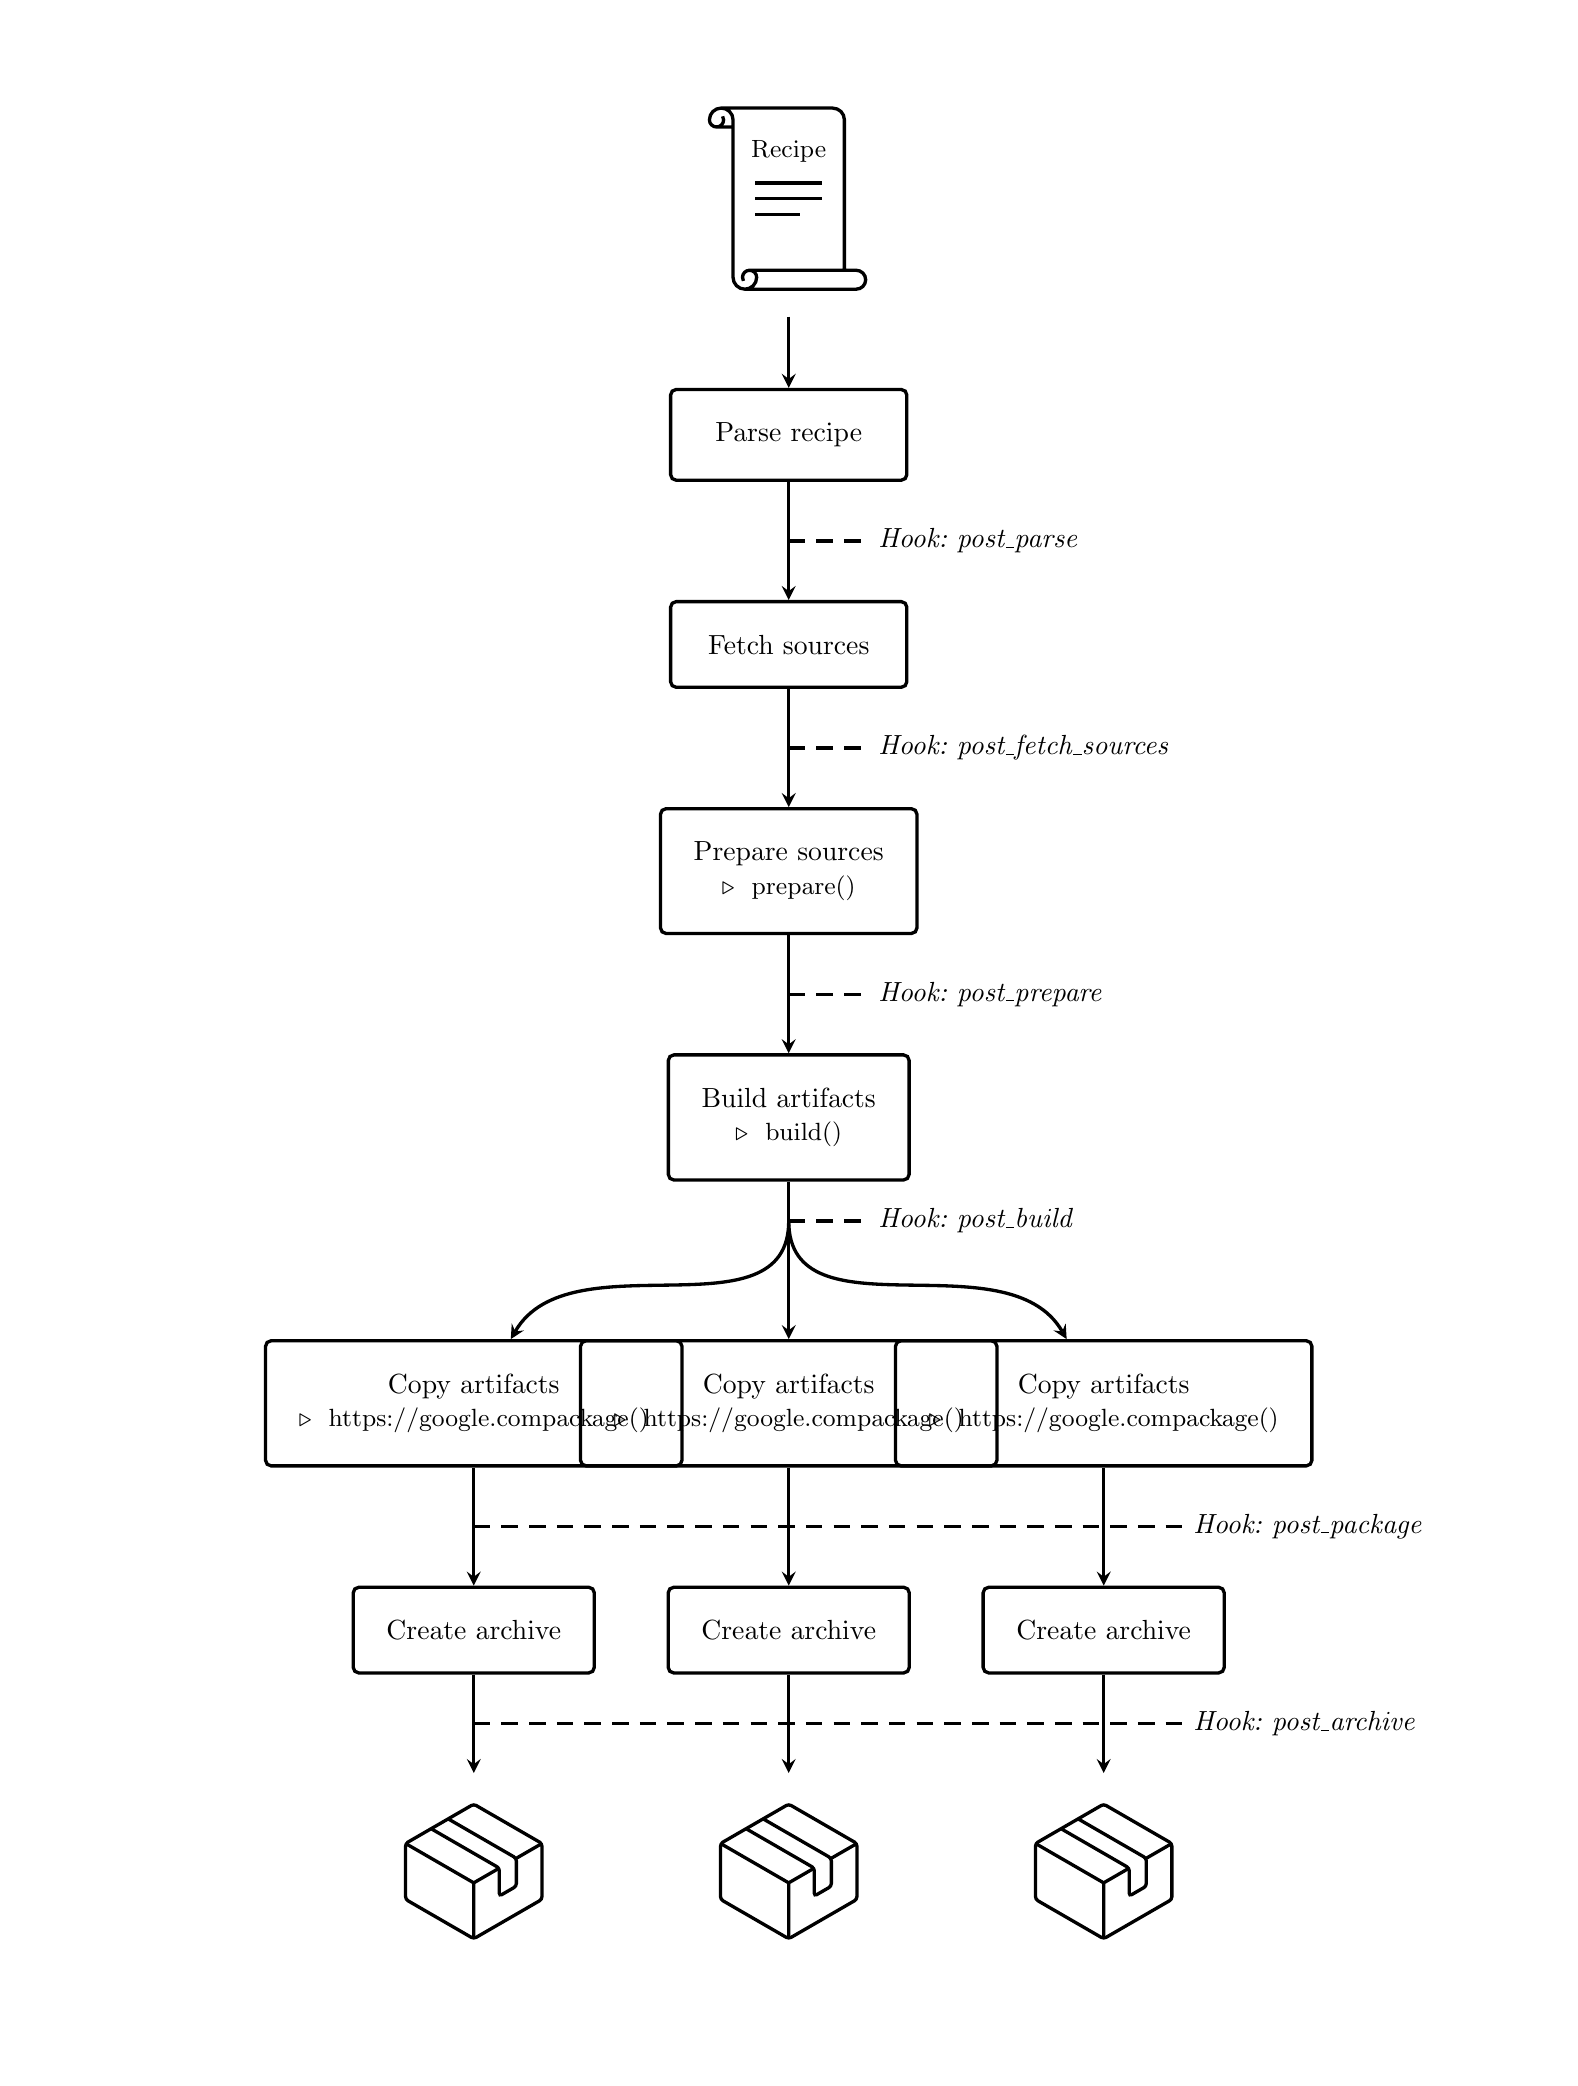
\begin{tikzpicture}[>=stealth, very thick, node distance=1.5cm]
    \pic[draw, pic text=\small Recipe]
        {scroll=1.414213562/2/.15};

    \node[process step] (parse) at (0, -3) {Parse recipe};
    \draw[arrow] (0, -1.5) -- (parse);

    \node[process step, below=of parse] (sources) {Fetch sources};
    \draw[arrow] (parse) -- (sources);
    \draw[hook line] ($(parse.south)!.5!(sources.north)$) -- ++(1, 0)
        node[hook] {post\_parse};

    \node[process step, below=of sources] (prepare) {
        Prepare sources\\
        \calls{prepare()}
    };
    \draw[arrow] (sources) -- (prepare);
    \draw[hook line] ($(sources.south)!.5!(prepare.north)$) -- ++(1, 0)
        node[hook] {post\_fetch\_sources};

    \node[process step, below=of prepare] (build) {
        Build artifacts\\
        \calls{build()}
    };
    \draw[arrow] (prepare) -- (build);
    \draw[hook line] ($(prepare.south)!.5!(build.north)$) -- ++(1, 0)
        node[hook] {post\_prepare};

    \foreach \i [evaluate=\i as \x using {(\i - 1) * 4cm}] in {0,1,2} {
        \node[process step, xshift=\x, below=2cm of build] (package-\i) {
            Copy artifacts\\
            \calls{\href{https://google.com}{package()}}
        };

        \node[process step, below=of package-\i] (archive-\i) {Create archive};

        \pic[draw] at ($(archive-\i.south)-(0, 2.5)$) {box=1/.71};
    }

    \draw (build.south) -- ++(0, -.5) coordinate (build-split);

    \draw[arrow] (build-split) to[out=-90, in=60] (package-0);
    \draw[arrow] (build-split) to (package-1);
    \draw[arrow] (build-split) to[out=-90, in=120] (package-2);

    \draw[arrow] (package-0) -- (archive-0);
    \draw[arrow] (package-1) -- (archive-1);
    \draw[arrow] (package-2) -- (archive-2);

    \draw[arrow] (archive-0.south) -- ++(0, -1.25) coordinate (final-0);
    \draw[arrow] (archive-1.south) -- ++(0, -1.25) coordinate (final-1);
    \draw[arrow] (archive-2.south) -- ++(0, -1.25) coordinate (final-2);

    \scoped[on background layer]{
        \fill[white] ($(current bounding box.north east)+(3cm, 1cm)$)
            rectangle ($(current bounding box.south west)-(3cm, 1cm)$);
    }

    \draw[hook line] (build-split) -- ++(1, 0)
        node[hook] {post\_build};

    \draw[hook line] ($(package-0.south)!.5!(archive-0.north)$)
        -- ($(package-1.south)!.5!(archive-1.north)$)
        -- ($(package-2.south)!.5!(archive-2.north)$)
        -- ++(1, 0) node[hook] {post\_package};

    \draw[hook line] ($(archive-0.south)!.5!(final-0)$)
        -- ($(archive-1.south)!.5!(final-1)$)
        -- ($(archive-2.south)!.5!(final-2)$)
        -- ++(1, 0) node[hook] {post\_archive};
\end{tikzpicture}
\end{document}
